\section{Introduction}
    \label{sec:intro}

    Le projet décrit dans ce rapport consiste à développer un logiciel d'analyse informatique des arbres d'attaque et de défense (\og Attack-Defense Trees \fg{} en anglais, ou ADTrees), nommé Glasir, dont le logo est présenté à la {\sc Figure}~\ref{fig:glasir}. Il intègrera entre autres un logiciel libre d'édition d'ADTrees déjà existant, ADTool, qui subira quelques modifications destinées à améliorer son ergonomie. Utilisé dans Glasir pour l'affichage, la création et l'édition des ADTrees, ADTool sera complété par les fonctionnalités d'analyse qui sont les suivantes :

    \begin{itemize}
    	\item le paramètre de synthèse, qui permet d'étendre le nombre de paramètres d'ADTool ;
    	\item le filtre, qui aide l'utilisateur à ôter de l’arbre les nœuds aux valuations hors d'un intervalle défini ;
    	\item l'optimiseur, qui sélectionne le meilleur chemin dans l'arbre selon une certaine valuation.
    \end{itemize} 

    Ce rapport de conception logicielle commencera par présenter l'architecture globale de Glasir, à l'aide d'un prototype d'interface et d'un diagramme de cas d'utilisation montrant les différentes actions accessibles à l'utilisateur. Cette présentation sera suivie d'un diagramme de classes général présentant l'architecture interne du logiciel. Enfin, le fonctionnement des modules principaux sera décrit par différents diagrammes de séquence, avant d'aborder les limites d'utilisation de Glasir.

    \begin{figure}[H]
        \centering
        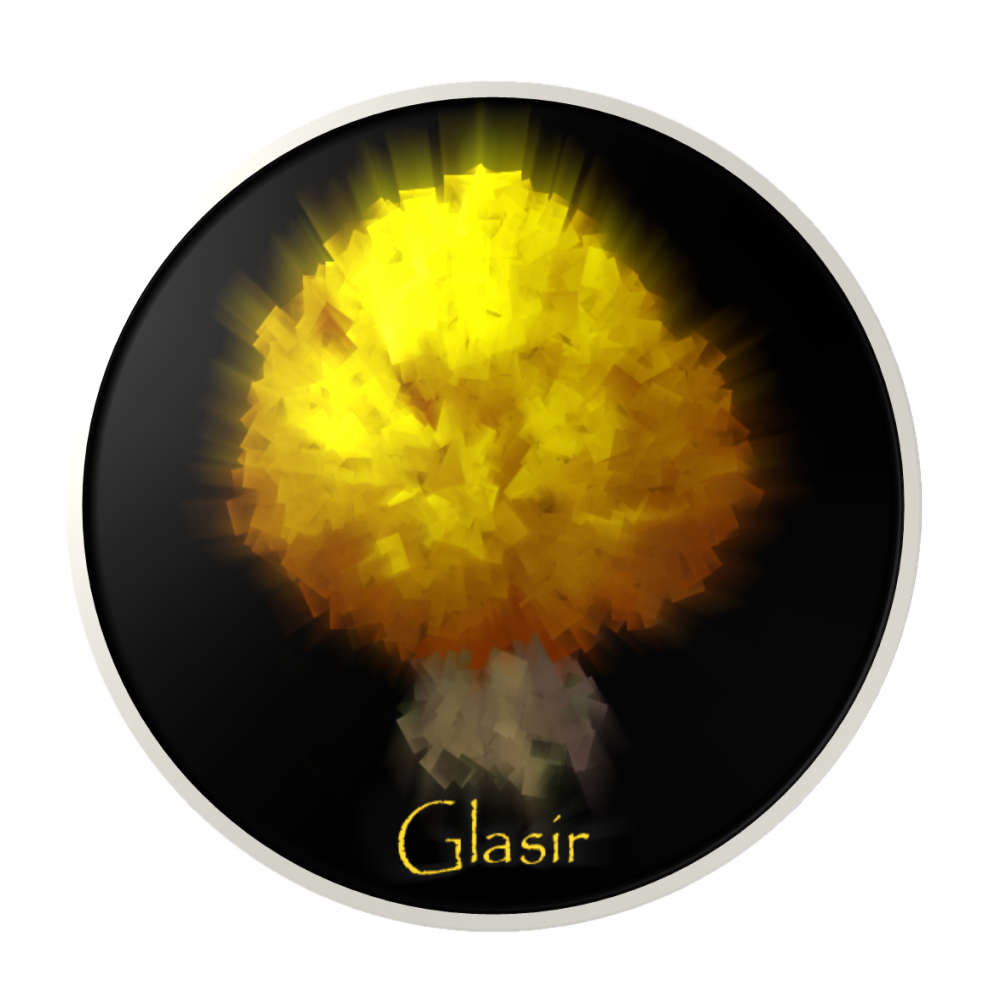
\includegraphics[height=0.5\textwidth]{figure/glasir.png}
        \caption{Logo du logiciel Glasir.}
        \label{fig:glasir}
    \end{figure}